% Options for packages loaded elsewhere
\PassOptionsToPackage{unicode}{hyperref}
\PassOptionsToPackage{hyphens}{url}
%
\documentclass[
  12pt,
]{article}
\title{Impacts of Dam Removal on the Shenandoah River}
\usepackage{etoolbox}
\makeatletter
\providecommand{\subtitle}[1]{% add subtitle to \maketitle
  \apptocmd{\@title}{\par {\large #1 \par}}{}{}
}
\makeatother
\subtitle{\url{https://github.com/lydiecos/WDA-Dam-Removal}}
\author{Lydie Costes}
\date{}

\usepackage{amsmath,amssymb}
\usepackage{lmodern}
\usepackage{iftex}
\ifPDFTeX
  \usepackage[T1]{fontenc}
  \usepackage[utf8]{inputenc}
  \usepackage{textcomp} % provide euro and other symbols
\else % if luatex or xetex
  \usepackage{unicode-math}
  \defaultfontfeatures{Scale=MatchLowercase}
  \defaultfontfeatures[\rmfamily]{Ligatures=TeX,Scale=1}
  \setmainfont[]{Times New Roman}
\fi
% Use upquote if available, for straight quotes in verbatim environments
\IfFileExists{upquote.sty}{\usepackage{upquote}}{}
\IfFileExists{microtype.sty}{% use microtype if available
  \usepackage[]{microtype}
  \UseMicrotypeSet[protrusion]{basicmath} % disable protrusion for tt fonts
}{}
\makeatletter
\@ifundefined{KOMAClassName}{% if non-KOMA class
  \IfFileExists{parskip.sty}{%
    \usepackage{parskip}
  }{% else
    \setlength{\parindent}{0pt}
    \setlength{\parskip}{6pt plus 2pt minus 1pt}}
}{% if KOMA class
  \KOMAoptions{parskip=half}}
\makeatother
\usepackage{xcolor}
\IfFileExists{xurl.sty}{\usepackage{xurl}}{} % add URL line breaks if available
\IfFileExists{bookmark.sty}{\usepackage{bookmark}}{\usepackage{hyperref}}
\hypersetup{
  pdftitle={Impacts of Dam Removal on the Shenandoah River},
  pdfauthor={Lydie Costes},
  hidelinks,
  pdfcreator={LaTeX via pandoc}}
\urlstyle{same} % disable monospaced font for URLs
\usepackage[margin=2.54cm]{geometry}
\usepackage{longtable,booktabs,array}
\usepackage{calc} % for calculating minipage widths
% Correct order of tables after \paragraph or \subparagraph
\usepackage{etoolbox}
\makeatletter
\patchcmd\longtable{\par}{\if@noskipsec\mbox{}\fi\par}{}{}
\makeatother
% Allow footnotes in longtable head/foot
\IfFileExists{footnotehyper.sty}{\usepackage{footnotehyper}}{\usepackage{footnote}}
\makesavenoteenv{longtable}
\usepackage{graphicx}
\makeatletter
\def\maxwidth{\ifdim\Gin@nat@width>\linewidth\linewidth\else\Gin@nat@width\fi}
\def\maxheight{\ifdim\Gin@nat@height>\textheight\textheight\else\Gin@nat@height\fi}
\makeatother
% Scale images if necessary, so that they will not overflow the page
% margins by default, and it is still possible to overwrite the defaults
% using explicit options in \includegraphics[width, height, ...]{}
\setkeys{Gin}{width=\maxwidth,height=\maxheight,keepaspectratio}
% Set default figure placement to htbp
\makeatletter
\def\fps@figure{htbp}
\makeatother
\setlength{\emergencystretch}{3em} % prevent overfull lines
\providecommand{\tightlist}{%
  \setlength{\itemsep}{0pt}\setlength{\parskip}{0pt}}
\setcounter{secnumdepth}{5}
\ifLuaTeX
  \usepackage{selnolig}  % disable illegal ligatures
\fi

\begin{document}
\maketitle

\begin{figure}
\centering
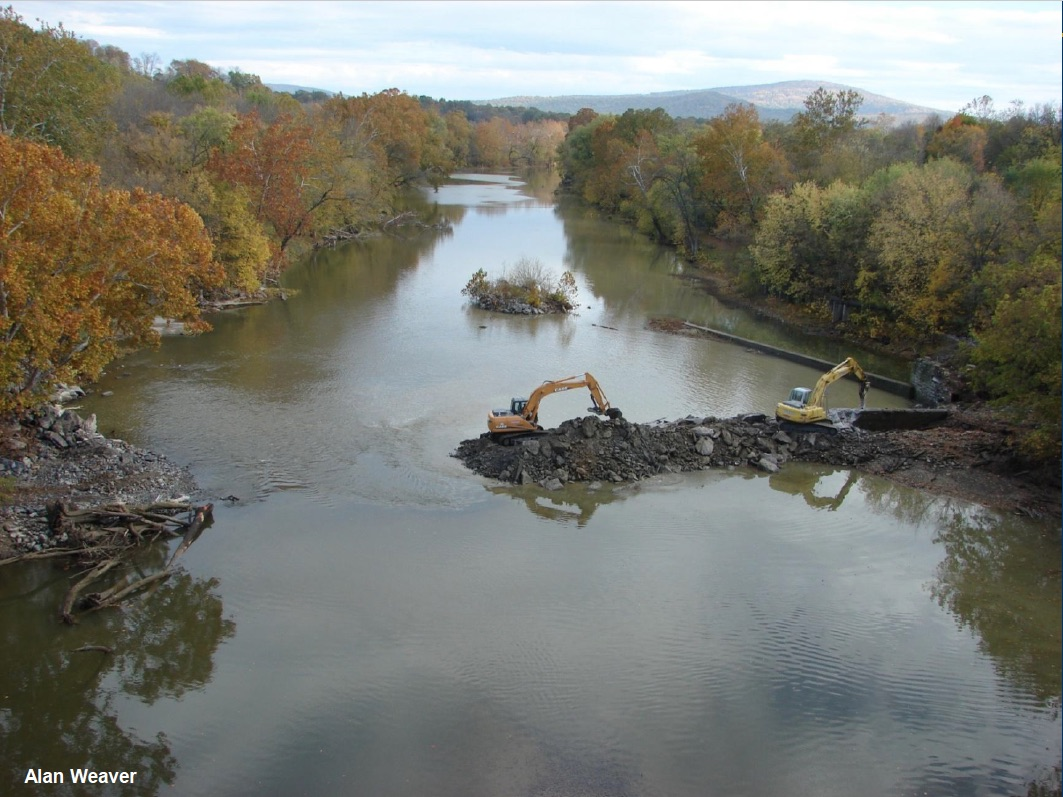
\includegraphics{Images/riverton-dam-removal.jpeg}
\caption{``Dam removal in progress on the North Fork of the Shenandoah
River''}
\end{figure}

\newpage
\tableofcontents 
\newpage
\listoftables 
\listoffigures 
\newpage

\hypertarget{rationale-and-research-questions}{%
\section{Rationale and Research
Questions}\label{rationale-and-research-questions}}

Over the past century, perceptions of dams have gradually changed, as
understanding of their serious ecological issues has increased and as
existing dams have aged, creating safety concerns and the need for
expensive repairs. Dams block the passage of fish and other aquatic
species, seriously disrupting life cycles for some species. They also
impact water quality and alter natural flow. Increasingly, dam removal
is pursued as an option to deal with aging dams and restore rivers.

In this study, I seek to understand how dam removal has impacted the
physical and chemical processes of one river, the Neuse River in North
Carolina. From 2004-2005, three dams were removed from the Southern Fork
of the Shenandoah River (see map below). The gage I will use for these
analyses is downstream from these dams and should thus reflect some of
the changes in flow and water quality that occurred after these
removals.

Below: The red X marks the spot of the McGaheysville Dam, which were
removed along with the Knightly Dam and Rockland Dam upstream in
2004-2005. All three dams were located along the south fork of the
Shenandoah River, which feeds into the Potomac.

\begin{figure}
\centering
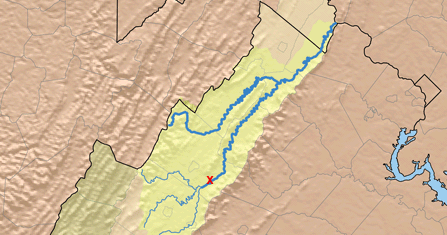
\includegraphics{../Figures-and-Maps/mcgaheysvilledam.png}
\caption{map of Neuse River}
\end{figure}

I am interested in both changes in physical process and changes in
chemical processes, which can vary widely according to the specific
river, its history, and the dam removal process (Foley et al 2017). Dams
allow for moderation of flow, often eliminating extreme flooding events.
Therefore, dam removal in combination with increasing extreme weather
events due to climate change could lead to more extreme and more
frequent high flow events. On the other hand, natural river systems and
riparian areas can be more resilient to flood events than artificially
constructed channels, so true restoration could help mitigate high flow
events to some extent.

Changes in water quality are also an area of interest. Large amounts of
sediment and minerals built up behind the dam may release quickly after
removal, especially if the removal was sudden rather than gradual (Foley
et al 2017). Over longer time, water quality is expected to improve
because of restored ecological processes.

\begin{enumerate}
\def\labelenumi{\arabic{enumi}.}
\item
  Question 1: Have discharge levels become more extreme since dam
  removal?
\item
  Question 2: Has there been a change in release of sediment and
  nutrients since the dam removal?
\end{enumerate}

\newpage

\hypertarget{dataset-information}{%
\section{Dataset Information}\label{dataset-information}}

The dataset consists of discharge and water quality data from stream
gage \#01631000, which is located on the South Fork of the Shenandoah
River downstream from the three dam removal sites. These data were
obtained from USGS StreamStats: \url{https://streamstats.usgs.gov/ss/}.

The dataset includes 183 parameters, but these parameters vary widely in
terms of how many datapoints were collected. To choose water quality
variables, I made a list of the top ten water quality parameters
according to the number of observations, and then selected three that I
thought would be particularly interesting and informative in light of
dam removal. These three were: suspended sediments, nitrogen, and
phosphate. Temperature is also included in the exploratory analyses. All
of these variables could be expected to change after dam removal.

\hypertarget{data-wrangling}{%
\subsection{Data Wrangling}\label{data-wrangling}}

The data were downloaded as two separate datasets: discharge
(`ShenaFlow') and water quality (`ShenaWQ'). Column names were changed
from defaults to be more comprehensible. Month and Year columns were
added to each dataset.

The discharge dataset was summarized into two dataframes, one by month
and the other by year. In both cases, discharge minimum, mean, and
maximum were calculated according to the summary unit.

The water quality dataset was transformed into a wider dataset with the
four parameters of interest divided into separate columns, instead of
being compiled in two columns by characteristic and value. The resulting
dataframe was also summarized by month, with minimum, mean, and maximum
calculated for each of the four parameters.

The exact timing of dam removal is unknown. Given that three dams were
removed between 2004-2005, subsequent analyses that compare ``before dam
removal'' versus ``after dam removal'' exclude the years 2004-2005
entirely. Most of the water quality variables did not include data for
these years anyway.

\begin{longtable}[]{@{}
  >{\raggedright\arraybackslash}p{(\columnwidth - 16\tabcolsep) * \real{0.17}}
  >{\raggedleft\arraybackslash}p{(\columnwidth - 16\tabcolsep) * \real{0.06}}
  >{\raggedleft\arraybackslash}p{(\columnwidth - 16\tabcolsep) * \real{0.07}}
  >{\raggedleft\arraybackslash}p{(\columnwidth - 16\tabcolsep) * \real{0.14}}
  >{\raggedleft\arraybackslash}p{(\columnwidth - 16\tabcolsep) * \real{0.14}}
  >{\raggedleft\arraybackslash}p{(\columnwidth - 16\tabcolsep) * \real{0.08}}
  >{\raggedleft\arraybackslash}p{(\columnwidth - 16\tabcolsep) * \real{0.11}}
  >{\raggedleft\arraybackslash}p{(\columnwidth - 16\tabcolsep) * \real{0.11}}
  >{\raggedleft\arraybackslash}p{(\columnwidth - 16\tabcolsep) * \real{0.12}}@{}}
\toprule
\begin{minipage}[b]{\linewidth}\raggedright
\end{minipage} & \begin{minipage}[b]{\linewidth}\raggedleft
vars
\end{minipage} & \begin{minipage}[b]{\linewidth}\raggedleft
n
\end{minipage} & \begin{minipage}[b]{\linewidth}\raggedleft
mean
\end{minipage} & \begin{minipage}[b]{\linewidth}\raggedleft
sd
\end{minipage} & \begin{minipage}[b]{\linewidth}\raggedleft
min
\end{minipage} & \begin{minipage}[b]{\linewidth}\raggedleft
max
\end{minipage} & \begin{minipage}[b]{\linewidth}\raggedleft
range
\end{minipage} & \begin{minipage}[b]{\linewidth}\raggedleft
se
\end{minipage} \\
\midrule
\endhead
Discharge & 1 & 33452 & 1602.8971960 & 2563.3337785 & 103.00 & 114000.00
& 113897.00 & 14.0150327 \\
Nitrogen\_mg.L & 1 & 588 & 0.9898299 & 0.4489218 & 0.01 & 2.69 & 2.68 &
0.0185132 \\
Phosphate\_mg.L & 2 & 581 & 0.2240637 & 0.2549325 & 0.00 & 1.93 & 1.93 &
0.0105764 \\
Sediments\_mg.L & 3 & 470 & 54.8588936 & 150.7588733 & 0.00 & 2020.00 &
2020.00 & 6.9539883 \\
\bottomrule
\end{longtable}

\newpage

\hypertarget{exploratory-analysis}{%
\section{Exploratory Analysis}\label{exploratory-analysis}}

Below are exploratory plots showing each parameter over time.

\begin{figure}
\centering
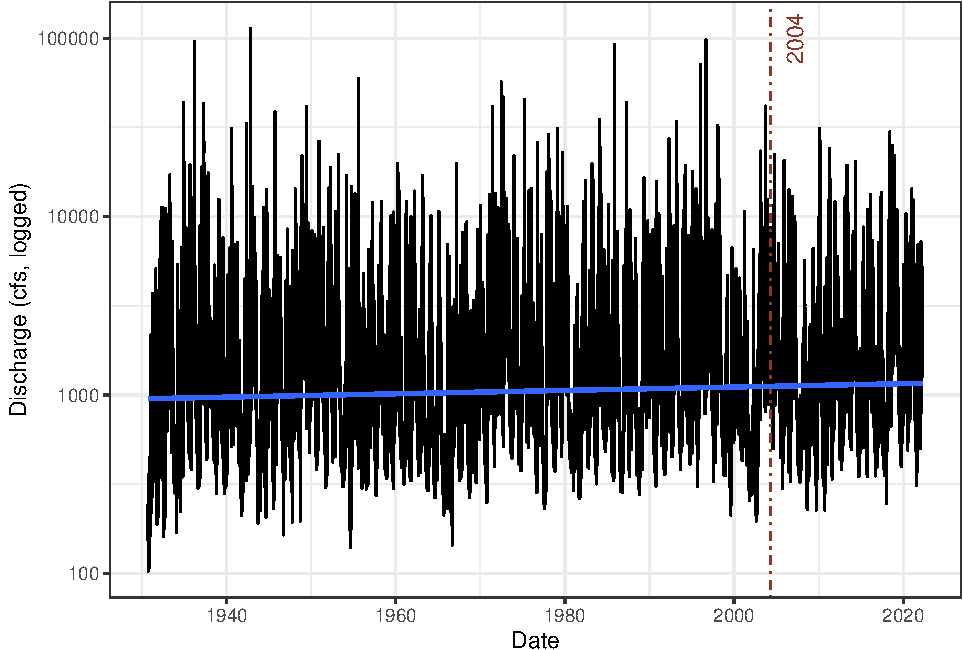
\includegraphics{Project_Script_files/figure-latex/exploration_plot1-1.pdf}
\caption{Discharge over time}
\end{figure}

\begin{figure}
\centering
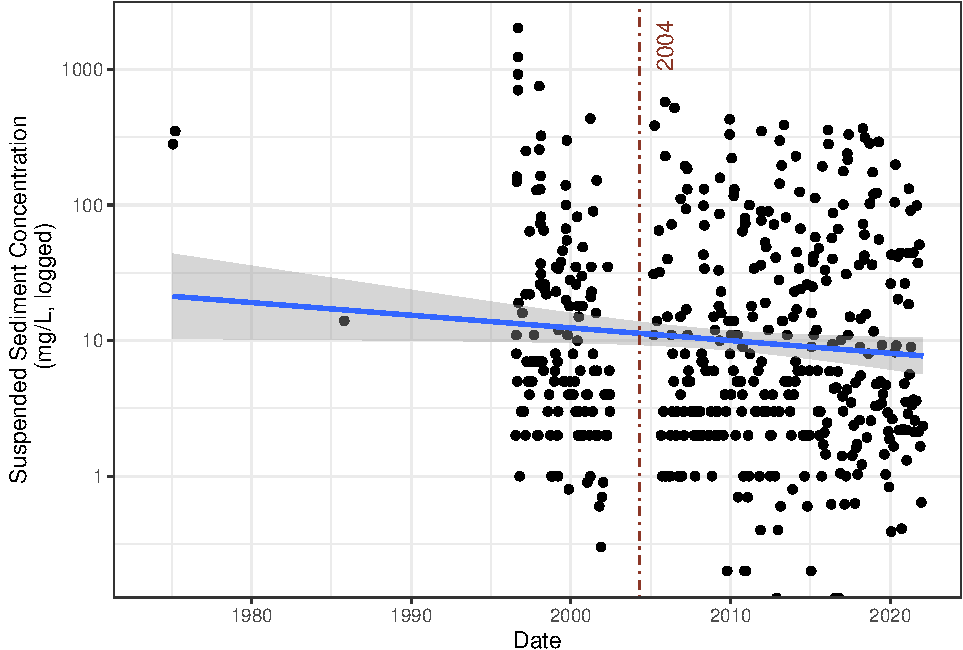
\includegraphics{Project_Script_files/figure-latex/exploration_plot2-1.pdf}
\caption{Sediment over time}
\end{figure}

\begin{figure}
\centering
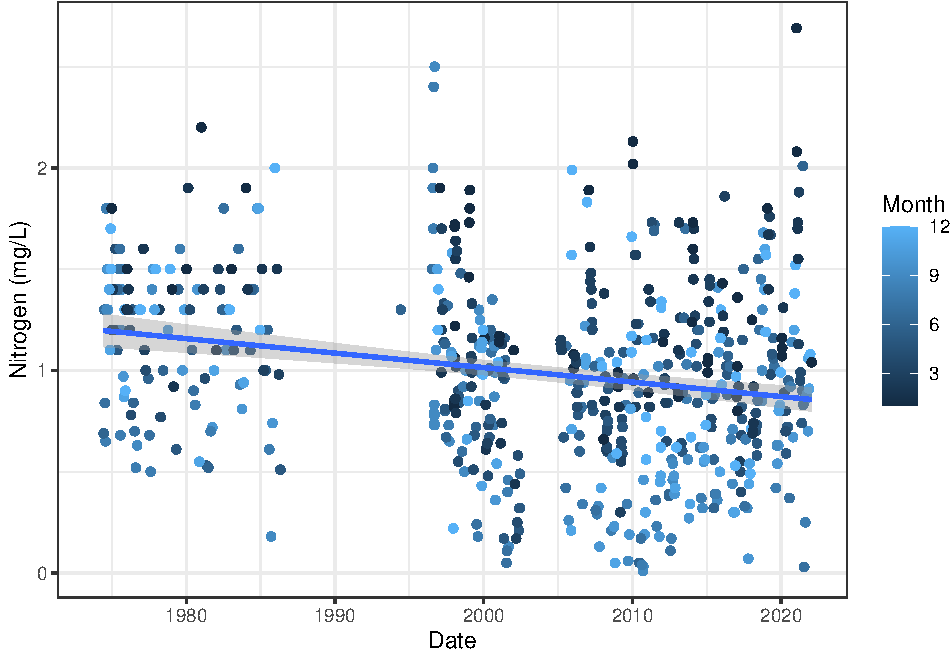
\includegraphics{Project_Script_files/figure-latex/exploration_plot3-1.pdf}
\caption{Nitrogen over time}
\end{figure}

\begin{figure}
\centering
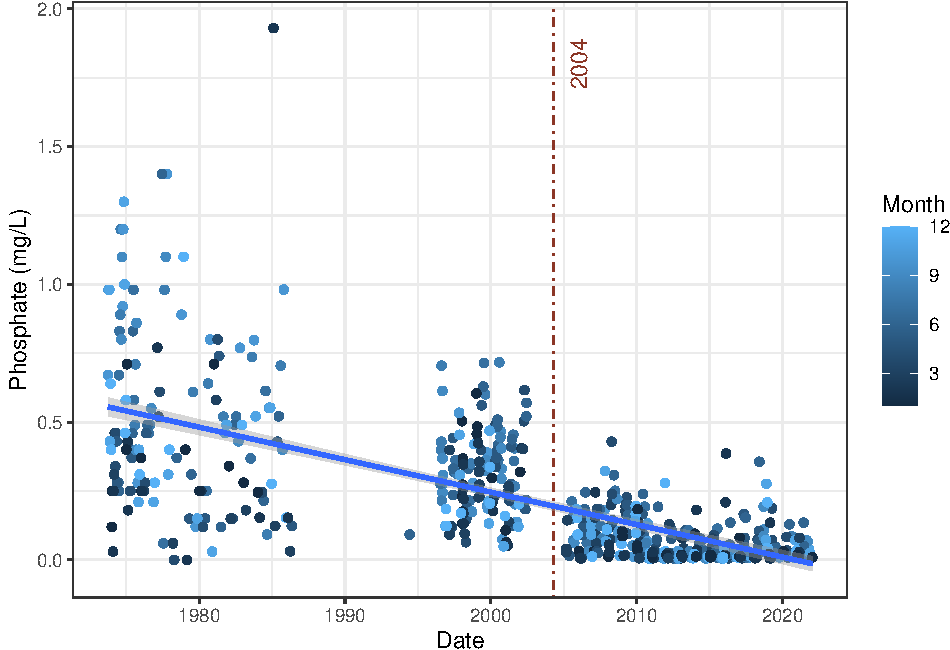
\includegraphics{Project_Script_files/figure-latex/exploration_plot4-1.pdf}
\caption{Phosphate over time}
\end{figure}

\newpage

\hypertarget{analysis}{%
\section{Analysis}\label{analysis}}

\hypertarget{part-1-flow}{%
\subsection{Part 1: Flow}\label{part-1-flow}}

\textbf{Question \#1: Have discharge extremes increased since the
removal of the dams? Has average discharge changed since dam removal?}

View minimum and maximum flow by month over time. The y-axis is logged
to more easily view the distribution of values.

\begin{figure}
\centering
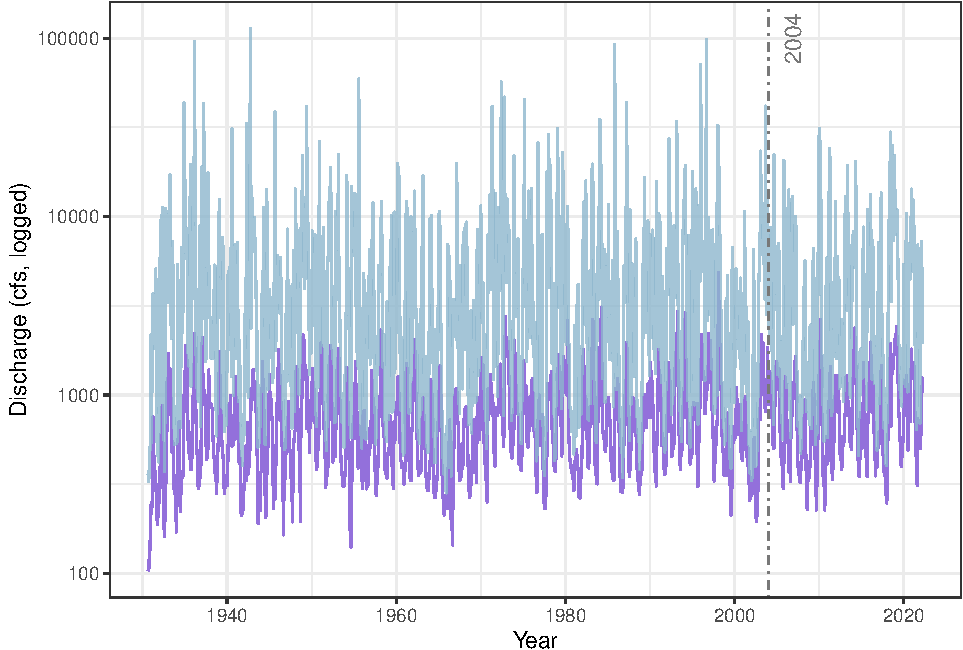
\includegraphics{Project_Script_files/figure-latex/Flow.analysis-1.pdf}
\caption{Monthly Minimum and Maximum Discharge Over Time}
\end{figure}

To better visualize extremes, we'll now look at minimum and maximum flow
along with average flow by year. Again, the y-axis is logged to aid with
visualization.

\begin{figure}
\centering
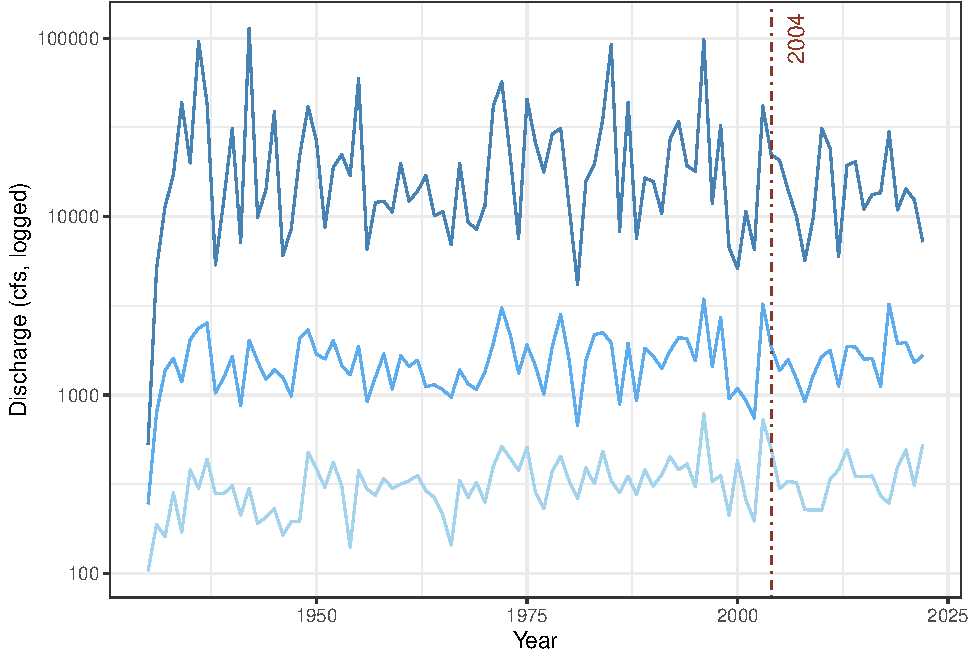
\includegraphics{Project_Script_files/figure-latex/Flow.analysis1-1.pdf}
\caption{Yearly Minimum, Maximum, and Average Discharge Over Time}
\end{figure}

These two graphs both suggest that maximum and minimum flows have not
gotten more extreme since dam removal; in fact, they appear to be less
extreme.

\newpage

\begin{longtable}[]{@{}llrrrrrrr@{}}
\caption{Summary Statistics for Discharge}\tabularnewline
\toprule
& Timeframe & n & mean & sd & min & max & range & se \\
\midrule
\endfirsthead
\toprule
& Timeframe & n & mean & sd & min & max & range & se \\
\midrule
\endhead
X1 & Before & 26764 & 1594.155 & 2687.319 & 103 & 114000 & 113897 &
16.42645 \\
X11 & After & 5957 & 1640.320 & 2009.289 & 226 & 31300 & 31074 &
26.03326 \\
\bottomrule
\end{longtable}

This table confirms that the river has not experienced more extreme
discharge events since dam removal. Additionally, average flow appears
to be higher since dam removal. Verify with a t-test:

\begin{verbatim}
## 
##  Welch Two Sample t-test
## 
## data:  ShenaFlow.before$Discharge and ShenaFlow.after$Discharge
## t = -1.4997, df = 11246, p-value = 0.1337
## alternative hypothesis: true difference in means is not equal to 0
## 95 percent confidence interval:
##  -106.50483   14.17313
## sample estimates:
## mean of x mean of y 
##  1594.155  1640.320
\end{verbatim}

Flow levels have not been significantly different before (\emph{M} =
1594.2, \emph{SD} = 2687.3) versus after (\emph{M} = 1640.3, \emph{SD} =
2009.5) the dam removal (\emph{p} = 0.140, \emph{t}(11202) = -1.48).

\newpage

We can view overall trends by running a time series that takes
seasonality into account. In the resulting graph, below, we see general
trend before the dam removal in red and after the dam removal in purple.

\begin{figure}
\centering
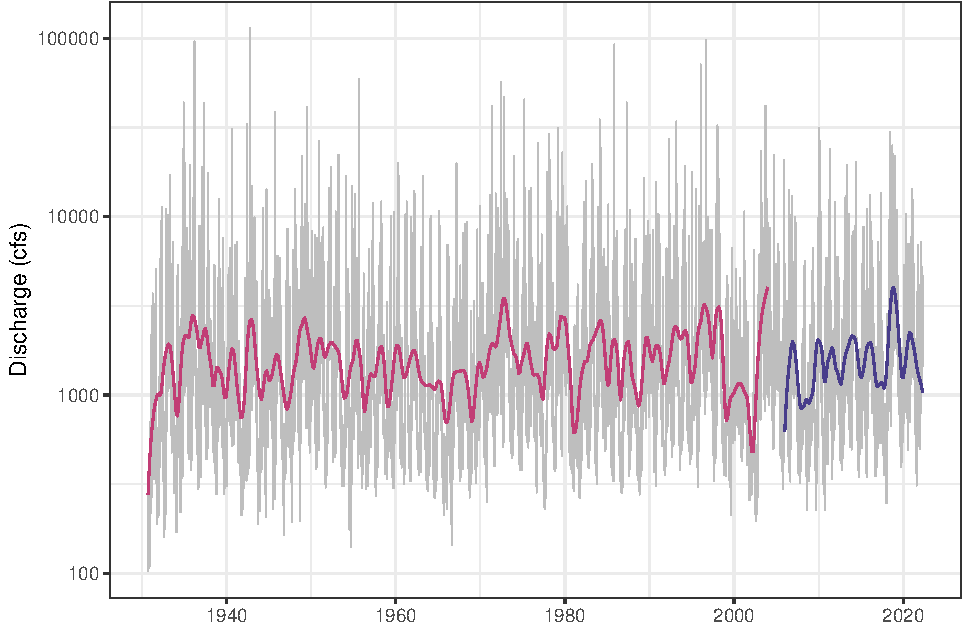
\includegraphics{Project_Script_files/figure-latex/flow_ts_graph-1.pdf}
\caption{Flow Trends Over Time}
\end{figure}

\newpage

\hypertarget{part-2}{%
\subsection{Part 2}\label{part-2}}

\textbf{Question \#2: Has there been a change in release of sediment and
nutrients since the dam removal?}

\hypertarget{sediment}{%
\subsubsection{Sediment}\label{sediment}}

\textbf{Have sediment levels changed since dam removal?}

View summary statistics comparing sediment levels before versus after
dam removal:

\begin{longtable}[]{@{}llrrrrrrr@{}}
\caption{Summary Statistics for Sediment}\tabularnewline
\toprule
& Timeframe & n & mean & sd & min & max & range & se \\
\midrule
\endfirsthead
\toprule
& Timeframe & n & mean & sd & min & max & range & se \\
\midrule
\endhead
Sediments\_mg.L & Before & 137 & 83.15474 & 242.94443 & 0.3 & 2020 &
2019.7 & 20.756144 \\
Sediments\_mg.L1 & After & 320 & 40.74525 & 79.73761 & 0.0 & 521 & 521.0
& 4.457468 \\
\bottomrule
\end{longtable}

Sediment levels appear to be lower on average since dam removal.

Test whether average sediment has been significantly different before
versus after dam removal:

\begin{verbatim}
## 
##  Welch Two Sample t-test
## 
## data:  ShenaWQ.before$Sediments_mg.L and ShenaWQ.after$Sediments_mg.L
## t = 1.9977, df = 148.7, p-value = 0.04758
## alternative hypothesis: true difference in means is not equal to 0
## 95 percent confidence interval:
##   0.4592669 84.3597221
## sample estimates:
## mean of x mean of y 
##  83.15474  40.74525
\end{verbatim}

Yes, sediment levels have been significantly different (\emph{t}(148.63)
= 2.00, \emph{p} = 0.047). Specifically, they have been lower post-dam
removal (\emph{M} = 40.64, \emph{SD} = 79.63) compared with pre-dam
removal (\emph{M}= 83.15, \emph{SD} = 242.94).

\newpage

\hypertarget{nitrogen}{%
\subsubsection{Nitrogen}\label{nitrogen}}

\textbf{Have nitrogen levels changed since dam removal?}

View summary statistics comparing nitrogen levels before versus after
dam removal:

\begin{longtable}[]{@{}llrrrrrrr@{}}
\caption{Summary Statistics for Nitrogen}\tabularnewline
\toprule
& Timeframe & n & mean & sd & min & max & range & se \\
\midrule
\endfirsthead
\toprule
& Timeframe & n & mean & sd & min & max & range & se \\
\midrule
\endhead
Nitrogen\_mg.L & Before & 254 & 1.0861811 & 0.4326022 & 0.05 & 2.50 &
2.45 & 0.0271439 \\
Nitrogen\_mg.L1 & After & 322 & 0.9156832 & 0.4456914 & 0.01 & 2.69 &
2.68 & 0.0248374 \\
\bottomrule
\end{longtable}

Visualize yearly minimum, mean, and maximum nitrogen levels:

\begin{figure}
\centering
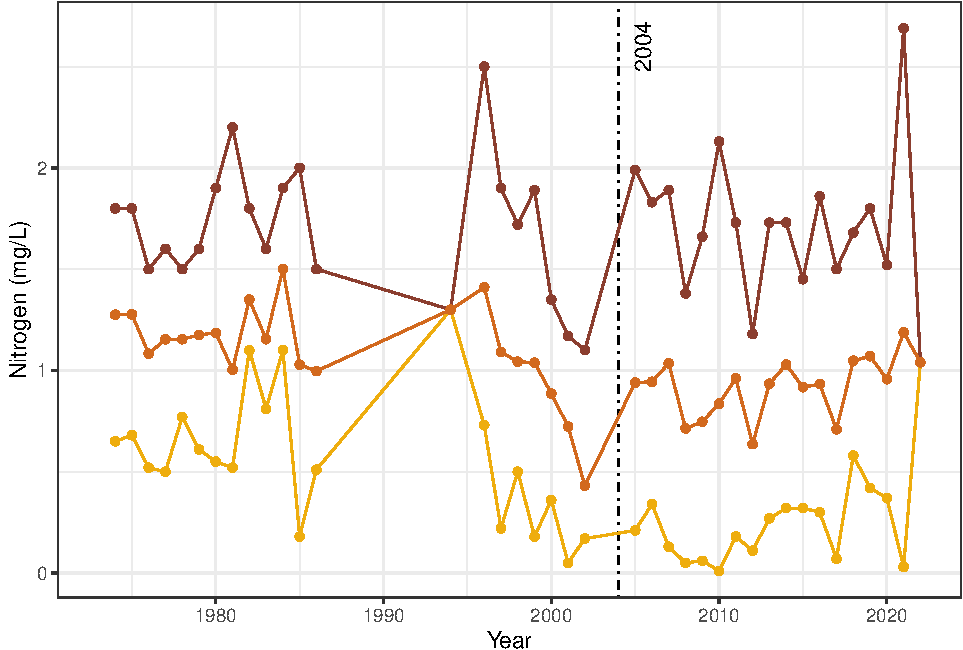
\includegraphics{Project_Script_files/figure-latex/Nitrogen_Analysis3-1.pdf}
\caption{Yearly Minimum, Maximum, and Average Nitrogen Levels Over Time}
\end{figure}

Check whether average nitrogen levels have changed since dam removal:

\begin{verbatim}
## 
##  Welch Two Sample t-test
## 
## data:  ShenaWQ.before$Nitrogen_mg.L and ShenaWQ.after$Nitrogen_mg.L
## t = 4.634, df = 550.09, p-value = 0.000004482
## alternative hypothesis: true difference in means is not equal to 0
## 95 percent confidence interval:
##  0.09822692 0.24276883
## sample estimates:
## mean of x mean of y 
## 1.0861811 0.9156832
\end{verbatim}

Yes, nitrogen levels since dam removal (\emph{M} = 0.92, \emph{SD} =
0.45) have been significantly lower (\emph{t}(550.8) = 4.56, \emph{p}
\textless{} 0.001) compared with nitrogen levels before dam removal
(\emph{M} = 1.09, \emph{SD} = 0.43).

\newpage

\hypertarget{phosphate}{%
\subsubsection{Phosphate}\label{phosphate}}

\textbf{Have phosphate levels changed since dam removal?}

View summary statistics comparing phosphate levels before versus after
dam removal:

\begin{longtable}[]{@{}llrrrrrrr@{}}
\caption{Summary Statistics for Phosphate}\tabularnewline
\toprule
& Timeframe & n & mean & sd & min & max & range & se \\
\midrule
\endfirsthead
\toprule
& Timeframe & n & mean & sd & min & max & range & se \\
\midrule
\endhead
Phosphate\_mg.L & Before & 272 & 0.3984853 & 0.2743858 & 0.000 & 1.930 &
1.930 & 0.0166371 \\
Phosphate\_mg.L1 & After & 296 & 0.0687061 & 0.0750149 & 0.006 & 0.429 &
0.423 & 0.0043602 \\
\bottomrule
\end{longtable}

Visualize yearly minimum, mean, and maximum phosphate levels:

\begin{figure}
\centering
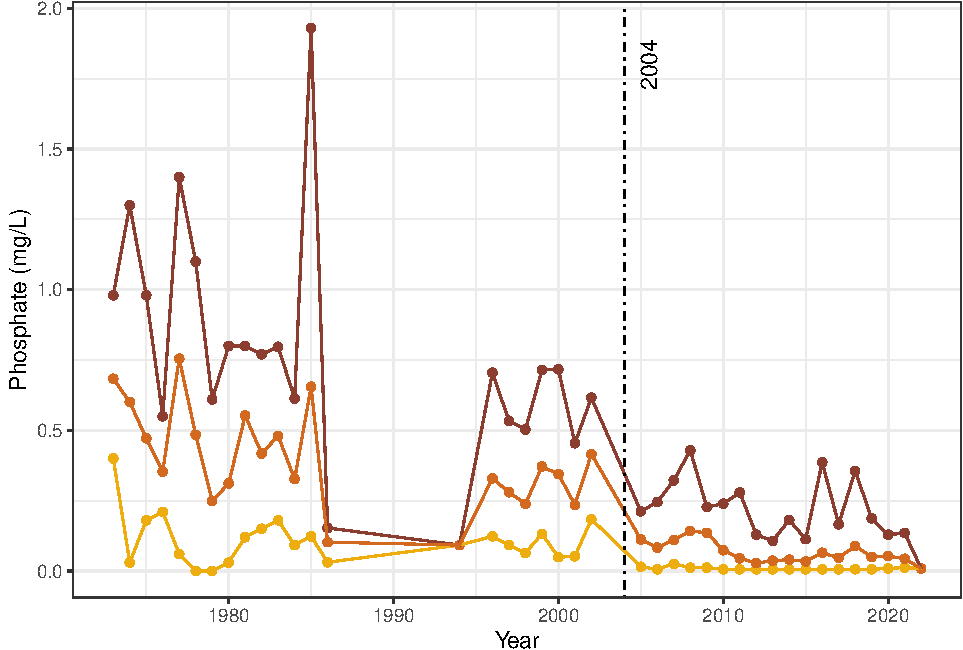
\includegraphics{Project_Script_files/figure-latex/Phosphate_Analysis3-1.pdf}
\caption{Yearly Minimum, Maximum, and Average Phosphate Levels Over
Time}
\end{figure}

Test whether phosphate levels were different before versus after dam
removal:

\begin{verbatim}
## 
##  Welch Two Sample t-test
## 
## data:  ShenaWQ.before$Phosphate_mg.L and ShenaWQ.after$Phosphate_mg.L
## t = 19.174, df = 308.17, p-value < 2.2e-16
## alternative hypothesis: true difference in means is not equal to 0
## 95 percent confidence interval:
##  0.2959370 0.3636214
## sample estimates:
##  mean of x  mean of y 
## 0.39848529 0.06870608
\end{verbatim}

Phosphate levels have been significantly lower (\emph{t}(309.22) =
19.10, \emph{p} \textless{} 0.001) since dam removal (\emph{M} = 0.07,
\emph{SD} = 0.08) compared with during the dammed years (\emph{M} =
0.40, \emph{SD} = 0.27).

\newpage

\hypertarget{summary-and-conclusions}{%
\section{Summary and Conclusions}\label{summary-and-conclusions}}

These findings suggest that the dam removals on the South Fork of the
Shenandoah did impact the flow, sediments, and nutrients of the river
downstream. Following these variables over a longer time window would
help explain the relative role of the dam removal itself compared with
changing climate factors, development, and other river impacts.

Because we did not know the exact timing of the three dam removals and
did not have data during these events for all variable, it is important
to differentiate between the immediate impacts of a dam removal versus
the longer term recovery of the hydrology and ecosystem. In general, dam
removal tends to cause a large release of sediment that has built up
behind the dam over the years, which may bring high levels of nutrients
as well (Stanley \& Doyle, 2002).

\textbf{Flow.} Average discharge levels have not changed since dam
removal, but the extremes of discharge have been smaller, both less
extreme high flow events and less extreme low flow events. This finding
is interesting because dams allow control of water, which could hedge
against both high and low flow events. On the other hand, restoring
natural hydrology makes rivers more resilient to extreme precipitation
and drought. The latter seems to be more important in this case, though
we cannot eliminate the possibility that perhaps there have not been as
extreme precipitation events nor droughts in the past 15 years compared
with prior decades. Further monitoring is needed.

\textbf{Sediment.} Sediment levels have been significantly lower since
removal. Data are not available for the year 2004, so we do not know the
degree of sediment release during and immediately after dam removal.
Past research has shown that the high release of sediment from a dam
removal can have significant impacts as far as coastal ecosystems (Rubin
et al., 2017). In this case at least, it seems that after the initial
release of sediment, the restoration of healthy river functions was able
to capture and hold a higher level of sediment.

\textbf{Nutrients.} Both nitrogen and phosphate levels have been
significantly lower since dam removal. In both cases, the decline in
nutrients appears to have begun before dam removal, and we did not
assess nutrient levels upstream of the dam over time. Therefore, we
cannot say definitively what role the dam itself played. The release and
retention of nitrogen and phosphate levels in rivers are at least
partially determined by sediment (Stanley \& Doyle, 2002). Thus, the
decline in nutrients is likely impacted by the decreased amount of
sediment release with changing hydrology as healthy river functions were
restored.

In summary, the removal of these three dams on the South Shenandoah
appears to have decreased discharge extremes and levels of sediment and
nutrients during the 15 years after the 2-year dam removal period.
Viewing the data during the actual period of dam removal would be
illuminating. Examining other gages, both upstream of the dams and
further downstream, could help us understand changing processes.
Furthermore, following these parameters over a longer time period will
help solidify our understanding of the dam removal, especially with
regards to the impacts of climate change and other stressors. Dam
removal holds great promise for restoring healthy fluvial systems. Every
river is unique, so research must continue to be able to predict the
impacts of dam removal and the optimal ways to do so.

\newpage

\hypertarget{references}{%
\section{References}\label{references}}

\begin{itemize}
\item
  Foley, M. M., J. R. Bellmore, J. E. O'Connor, J. J. Duda, A. E. East,
  G. E. Grant, C. W. Anderson, J. A. Bountry, M. J. Collins, P. J.
  Connolly, L. S. Craig, J. E. Evans, S. L. Greene,F. J. Magilligan, C.
  S. Magirl, J. J. Major, G. R. Pess,T. J. Randle, P. B. Shafroth, C. E.
  Torgersen, D. Tullos, A. C. Wilcox. 2017. Dam removal: Listening in.
  \emph{Water Resources Research. 53}(7):5229-5246.
  \url{https://doi-org.proxy.lib.duke.edu/10.1002/2017WR020457}
\item
  Musser, K. Map. \emph{Fish Passage and Dam Removal.}
  \url{http://www.virginiaplaces.org/watersheds/fishpassage.html}
\item
  Rubin, S. P., Miller, I. M., Foley, M. M., Berry, H. D., Duda, J. J.,
  Hudson, B., et al.~(2017). Increased sediment load during a
  large-scale dam removal changes nearshore subtidal communities.
  \emph{PLoS ONE 12}(12): e0187742.
  \url{https://doi.org/10.1371/journal.pone.0187742}
\item
  Stanley, E. H., \& Doyle, M. W. (2002). A geomorphic perspective on
  nutrient retention following dam removal: geomorphic models provide a
  means of predicting ecosystem responses to dam removal.
  \emph{BioScience, 52}(8), 693+.
  \url{https://link.gale.com/apps/doc/A90317049/EAIM?u=duke_perkins\&sid=summon\&xid=26814f17}
\item
  U.S. Geological Survey. 2022. The StreamStats program.
  \url{https://streamstats.usgs.gov/ss/}
\item
  Virginia Department of Wildlife Resources. 2022. Fish Passage Program.
  \url{https://dwr.virginia.gov/fishing/fish-passage/\#potomac}
\item
  Weaver, A. 2010. Photograph. \emph{U.S. Fish and Wildlife Service
  Northeast Region.}
  \url{https://usfwsnortheast.wordpress.com/2016/12/13/virginia-rivers-opened-for-the-first-time-in-100-years/}
\end{itemize}

\end{document}
